\section{Regulador de voltaje}
Mientras los filtros pueden reducir la fluctuación de las fuentes de
alimentación, el método más efectivo es una combinación de un filtro de entrada
con capacitor utilizado con un regulador de voltaje. Se conecta un regulador de
voltaje a la salida de un rectificador filtrado y mantiene un voltaje de salida
constante. El filtro de entrada con capacitor reduce el rizo de entrada al
regulador a un nivel aceptable. La combinación de un capacitor grande y un
regulador de voltaje ayudan a producir una excelente fuente de alimentación.

\subsection{Diodo \emph{Zener}}
Cuando se polariza hacia atrás con un potencial suficientemente grande, el
comportamiento normal del diodo inverso (de un interruptor abierto) cambia
abruptamente para mantener un voltaje fijo; \textbf{el potencial \emph{Zener}}.
La corriente a través del diodo comienza a aumentar drásticamente una vez que se
alcanza este potencial. Si se coloca un diodo \emph{Zener} a través de la salida
del rectificador filtrado, el \emph{Zener} intentará limitar el voltaje
de salida al potencial \emph{Zener}.

Para evitar el consumo excesivo y posiblemente destructivo de corriente por el
diodo \emph{Zener}, la diferencia de voltaje entre el voltaje del condensador y
el potencial \emph{Zener} se reduce a través de una resistencia limitadora de
corriente en serie. Esta resistencia limitadora establecerá la cantidad máxima
de corriente de salida. Esta corriente se divide entonces entre el diodo
\emph{Zener} y la carga.

Bajo condiciones de carga ligera, la mayor parte de esta corriente fluirá a
través del diodo \emph{Zener}. Bajo condiciones de carga pesada, la mayor parte
de la corriente será extraída por la carga con poco flujo a través del diodo
\emph{Zener}. Si la demanda de corriente de carga es demasiado pesada, no hay
corriente disponible para el diodo \emph{Zener} y deja de conducir. La
regulación se pierde y la resistencia limitadora forma un divisor de voltaje con
la carga \cite{Fiore}.

\subsubsection{Calculo de la resistencia limitadora}
Considerando el voltaje de entrada:
\begin{equation*}
    \begin{split}
        V_i &= 18\,\sen(100\pi\,t)[\text{V}]\\
    \end{split}
\end{equation*}

Se utilizará un diodo \emph{Zener} \textbf{1N4742A} con los siguientes
parametros:
\begin{equation*}
    \begin{split}
        V_z &= 12[\text{V}]\\
        P_z &= 0.5[\text{W}]\\
    \end{split}
\end{equation*}

Se halla el intervalo aceptable de corriente:
\begin{equation*}
    \begin{split}
        I_{\text{max}} &= \frac{P_z}{V_z}\\
                       &= \frac{0.5}{12}\\
                       &= 41.67[\text{mA}]\\
        I_{\text{min}} &= 0.1\,I_{\text{max}}\\
                       &= 0.1\,41.67[\text{mA}]\\
                       &= 4.167[\text{mA}]\\
    \end{split}
\end{equation*}

Por tanto, los intervalos aceptables para la resistencia limitadora son:
\begin{equation*}
    \begin{split}
        R_{\text{max}} &= \frac{V_p - V_z}{I_{\text{max}}}\\
                       &= \frac{18 - 12}{0.041.67}\\
                       &= 144[\Omega]\\
        R_{\text{min}} &= \frac{V_p - V_z}{I_{\text{min}}}\\
                       &= \frac{18 - 12}{0.0041.67}\\
                       &= 1440[\Omega]\\
    \end{split}
\end{equation*}

El valor normalizado para la resistencia limitadora utilizado es
$1[\text{k}\Omega]$.

El circuito con filtro y con diodo \emph{Zener} puede verse en la
\textbf{figura~\ref{circuito08}}.

\begin{figure}[!h]
\centering
\includegraphics[scale=1.20]{diagramas/08.zener1.eps}
\caption{Regulación de voltaje con diodo \emph{Zener}.}
\label{circuito08}
\end{figure}

\subsubsection{Simulación}
Se utilizó el software \emph{Quite Universal Circuit Simulator.} versión 23.3.1
para la simulación de la regulación de voltaje con el diodo \emph{Zener}, este
puede verse en la \textbf{figura~\ref{simulacion08}}.

\begin{figure}[!h]
\centering
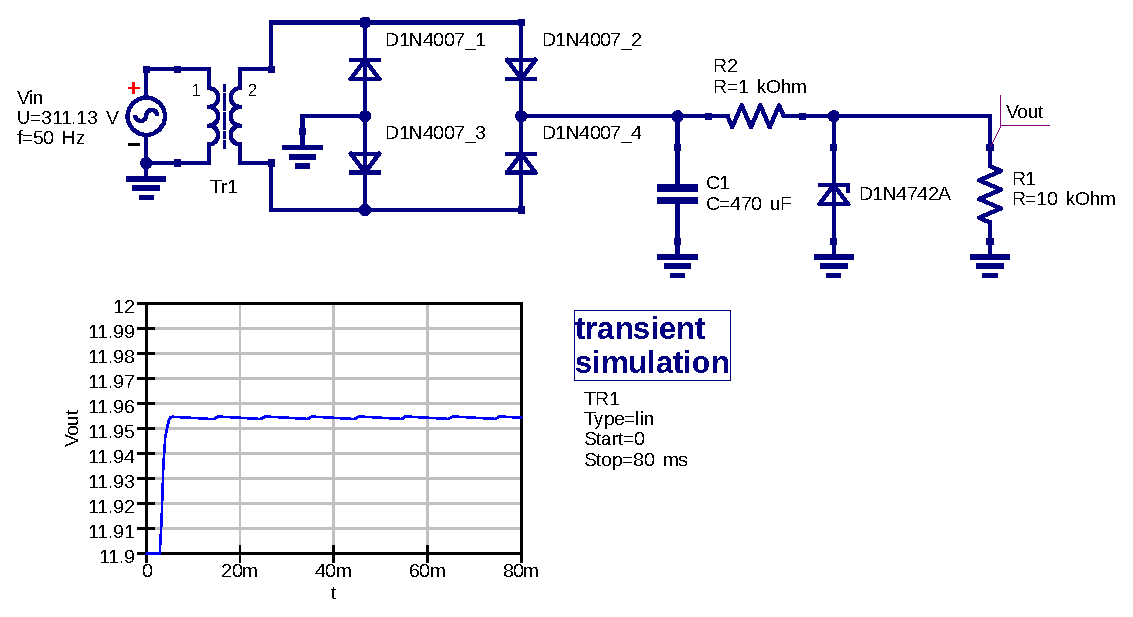
\includegraphics[scale=0.75]{simulacion/08.zener1.eps}
\caption{Simulación con el diodo \emph{Zener} \textbf{1N4742A}.}
\label{simulacion08}
\end{figure}

\subsubsection{Laboratorio}
Se presenta el regulador con diodo \emph{Zener} \textbf{1N4742A} armado en
laboratorio, su señal de voltaje de salida en osciloscopio, asi como el voltaje
de la carga y las corrientes en la resistencia limitadora de
$1[\text{k}\Omega]$, diodo \emph{Zener} y resistencia de carga de
$10[\text{k}\Omega]$ en la \textbf{figura~\ref{laboratorio10}}.

\begin{figure}[!h]
\centering
\includegraphics[scale=0.28]{fotos/08.zener1.eps}
\caption{Regulador con diodo \emph{Zener} \textbf{1N4742A}.}
\label{laboratorio10}
\end{figure}

\subsection{Regulador L78XX}
La mayoría de los reguladores son circuitos integrados y tienen tres terminales:
una de entrada, una de salida y una de referencia (o ajuste). Primero se filtra
la entrada al regulador con un capacitor para reducir el rizo a $<10\%$.
Típicamente, los reguladores de voltaje proporcionan una salida constante con un
alto rechazo a los rizos.

Los reguladores de tres terminales diseñados para voltajes de salida fijos
requieren sólo capacitores externos para completar la parte de regulación de la
fuente de alimentación. El filtrado se realiza por un capacitor de gran valor
entre el voltaje de entrada y tierra. Un capacitor de salida está conectado de
la salida a tierra para mejorar la respuesta transitoria \cite{Floyd}.

En la \textbf{figura~\ref{circuito09}} se muestra un circuito regulador
\textbf{L7809CV} que fija el voltaje a $+9[\text{V}]$ filtrado por un capacitor
de $470[\mu\text{F}]$ en la entrada y un capacitor de $10[\mu\text{F}]$ para la
salida.

\begin{figure}[!h]
\centering
\includegraphics[scale=1.20]{diagramas/09.regulador1.eps}
\caption{Regulación de voltaje \textbf{L7809CV}.}
\label{circuito09}
\end{figure}

\subsubsection{Simulación}
Se utilizó el software \emph{Quite Universal Circuit Simulator.} versión 23.3.1
para la simulación de la regulación de voltaje con el circuito integrado
\textbf{L7809CV} este puede verse en la \textbf{figura~\ref{simulacion09}}.

\begin{figure}[!h]
\centering
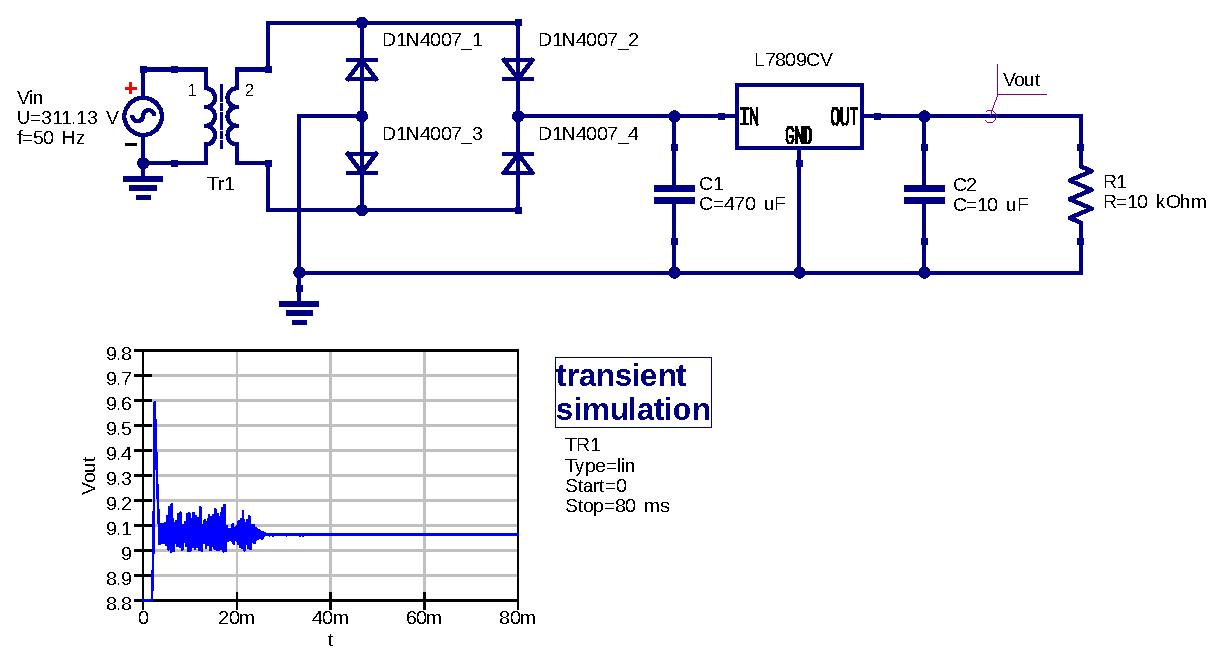
\includegraphics[scale=0.75]{simulacion/09.regulador1.eps}
\caption{Simulación del regulador \textbf{L7809CV}.}
\label{simulacion09}
\end{figure}

\subsubsection{Laboratorio}
Se presenta el regulador \textbf{L7809CV} armado en laboratorio, su señal de
voltaje de salida en osciloscopio, asi como su voltaje y corriente en un
multimetro para una resistencia de carga de $10[\text{k}\Omega]$ en la
\textbf{figura~\ref{laboratorio11}}.

\begin{figure}[!h]
\centering
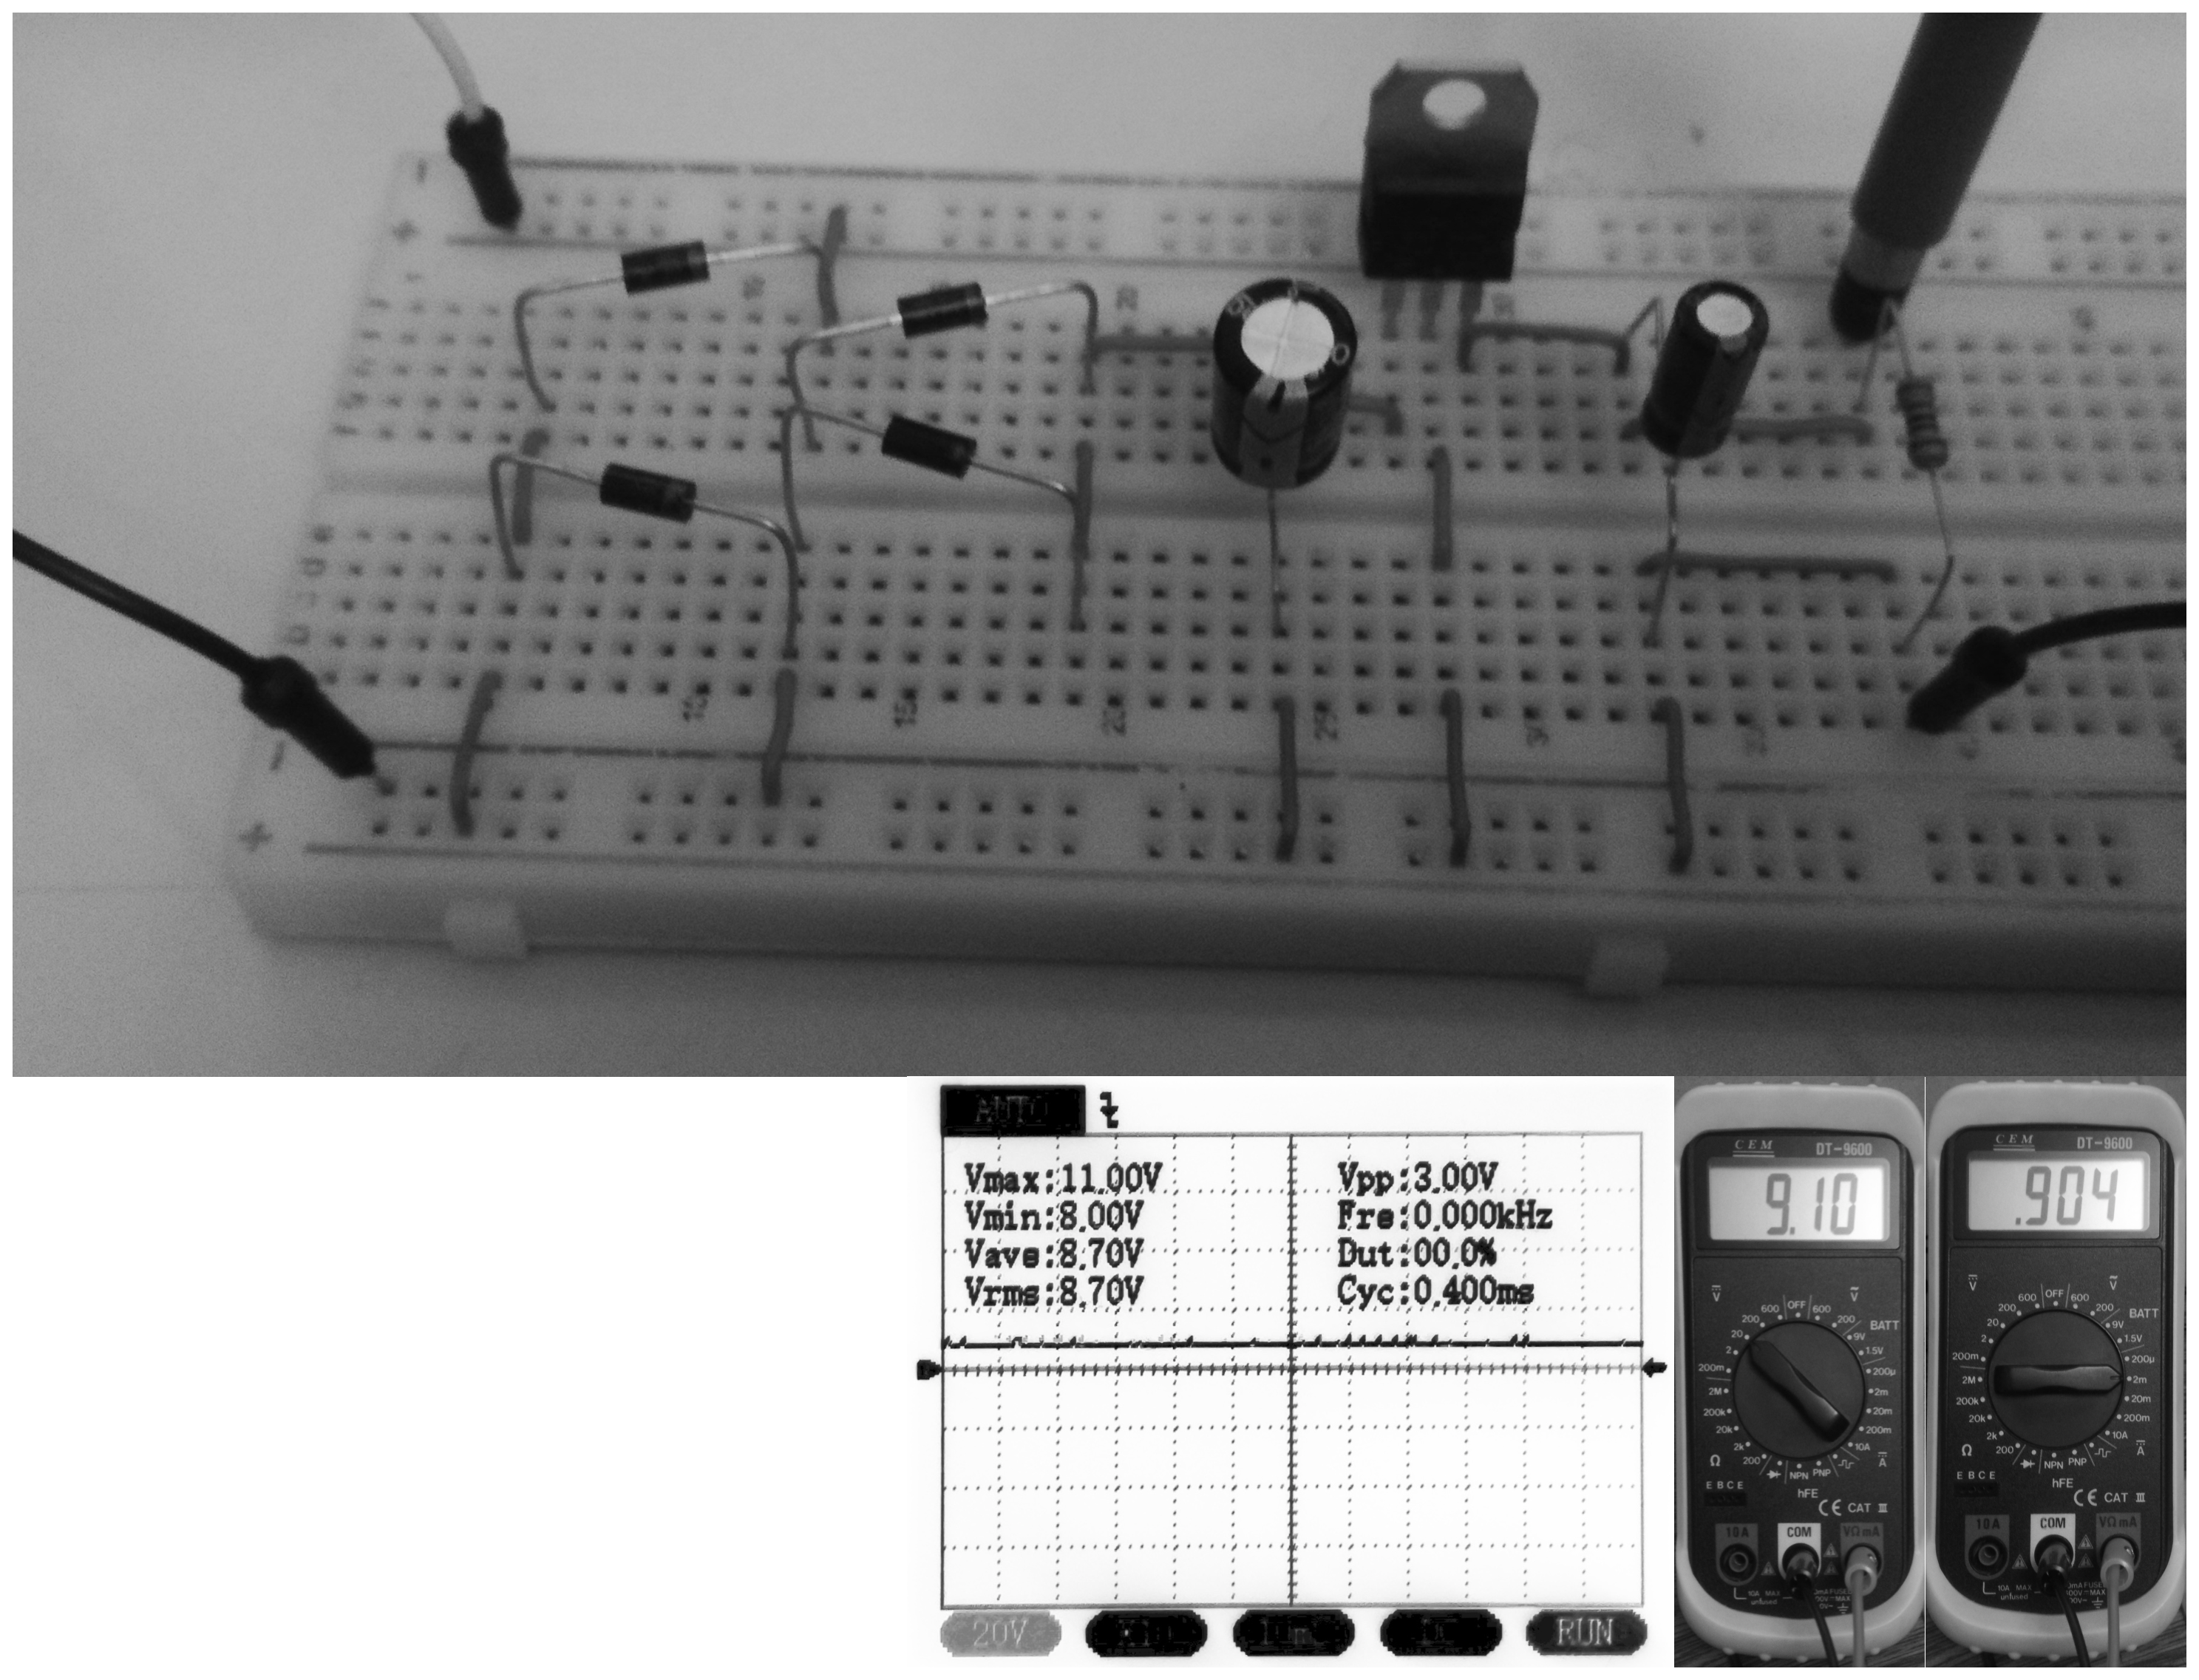
\includegraphics[scale=0.28]{fotos/09.regulador1.eps}
\caption{Regulador \textbf{L7809CV}, salida del osciloscopio\\
y medicion de voltaje y corriente.}
\label{laboratorio11}
\end{figure}

\subsection{Regulador L79XX}
Ademas de los reguladores anteriormente mencionados, tambien existen reguladores
de tipo negativo que proveen una salida de voltaje inverso.

En la \textbf{figura~\ref{circuito10}} se muestra un circuito regulador
\textbf{L7909CV} que fija el voltaje a $-9[\text{V}]$ filtrado por un capacitor
de $470[\mu\text{F}]$ en la entrada y un capacitor de $10[\mu\text{F}]$ para la
salida.

\begin{figure}[!h]
\centering
\includegraphics[scale=1.20]{diagramas/10.regulador2.eps}
\caption{Regulación de voltaje \textbf{L7909CV}.}
\label{circuito10}
\end{figure}

\subsubsection{Simulación}
Se utilizó el software \emph{Quite Universal Circuit Simulator.} versión 23.3.1
para la simulación de la regulación de voltaje con el circuito integrado
\textbf{L7909CV} este puede verse en la \textbf{figura~\ref{simulacion10}}.

\begin{figure}[!h]
\centering
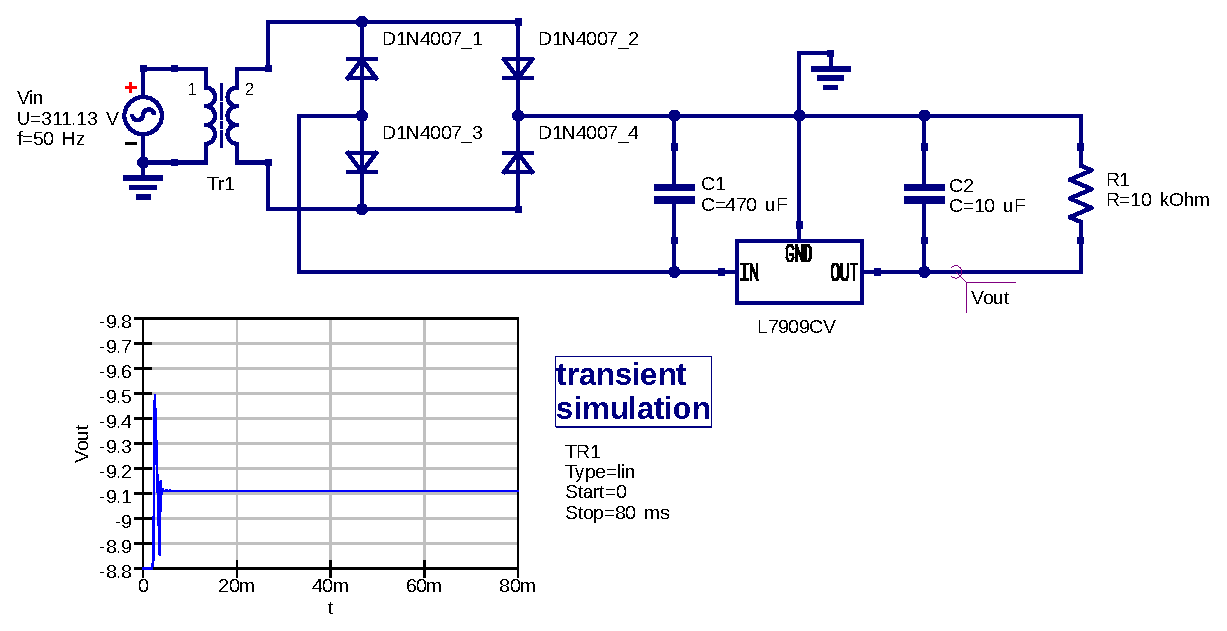
\includegraphics[scale=0.75]{simulacion/10.regulador2.eps}
\caption{Simulación del regulador \textbf{L7909CV}.}
\label{simulacion10}
\end{figure}

\subsubsection{Laboratorio}
Se presenta el regulador \textbf{L7909CV} armado en laboratorio, su señal de
voltaje de salida en osciloscopio, asi como su voltaje y corriente en un
multimetro para una resistencia de carga de $10[\text{k}\Omega]$ en la
\textbf{figura~\ref{laboratorio12}}.

\begin{figure}[!h]
\centering
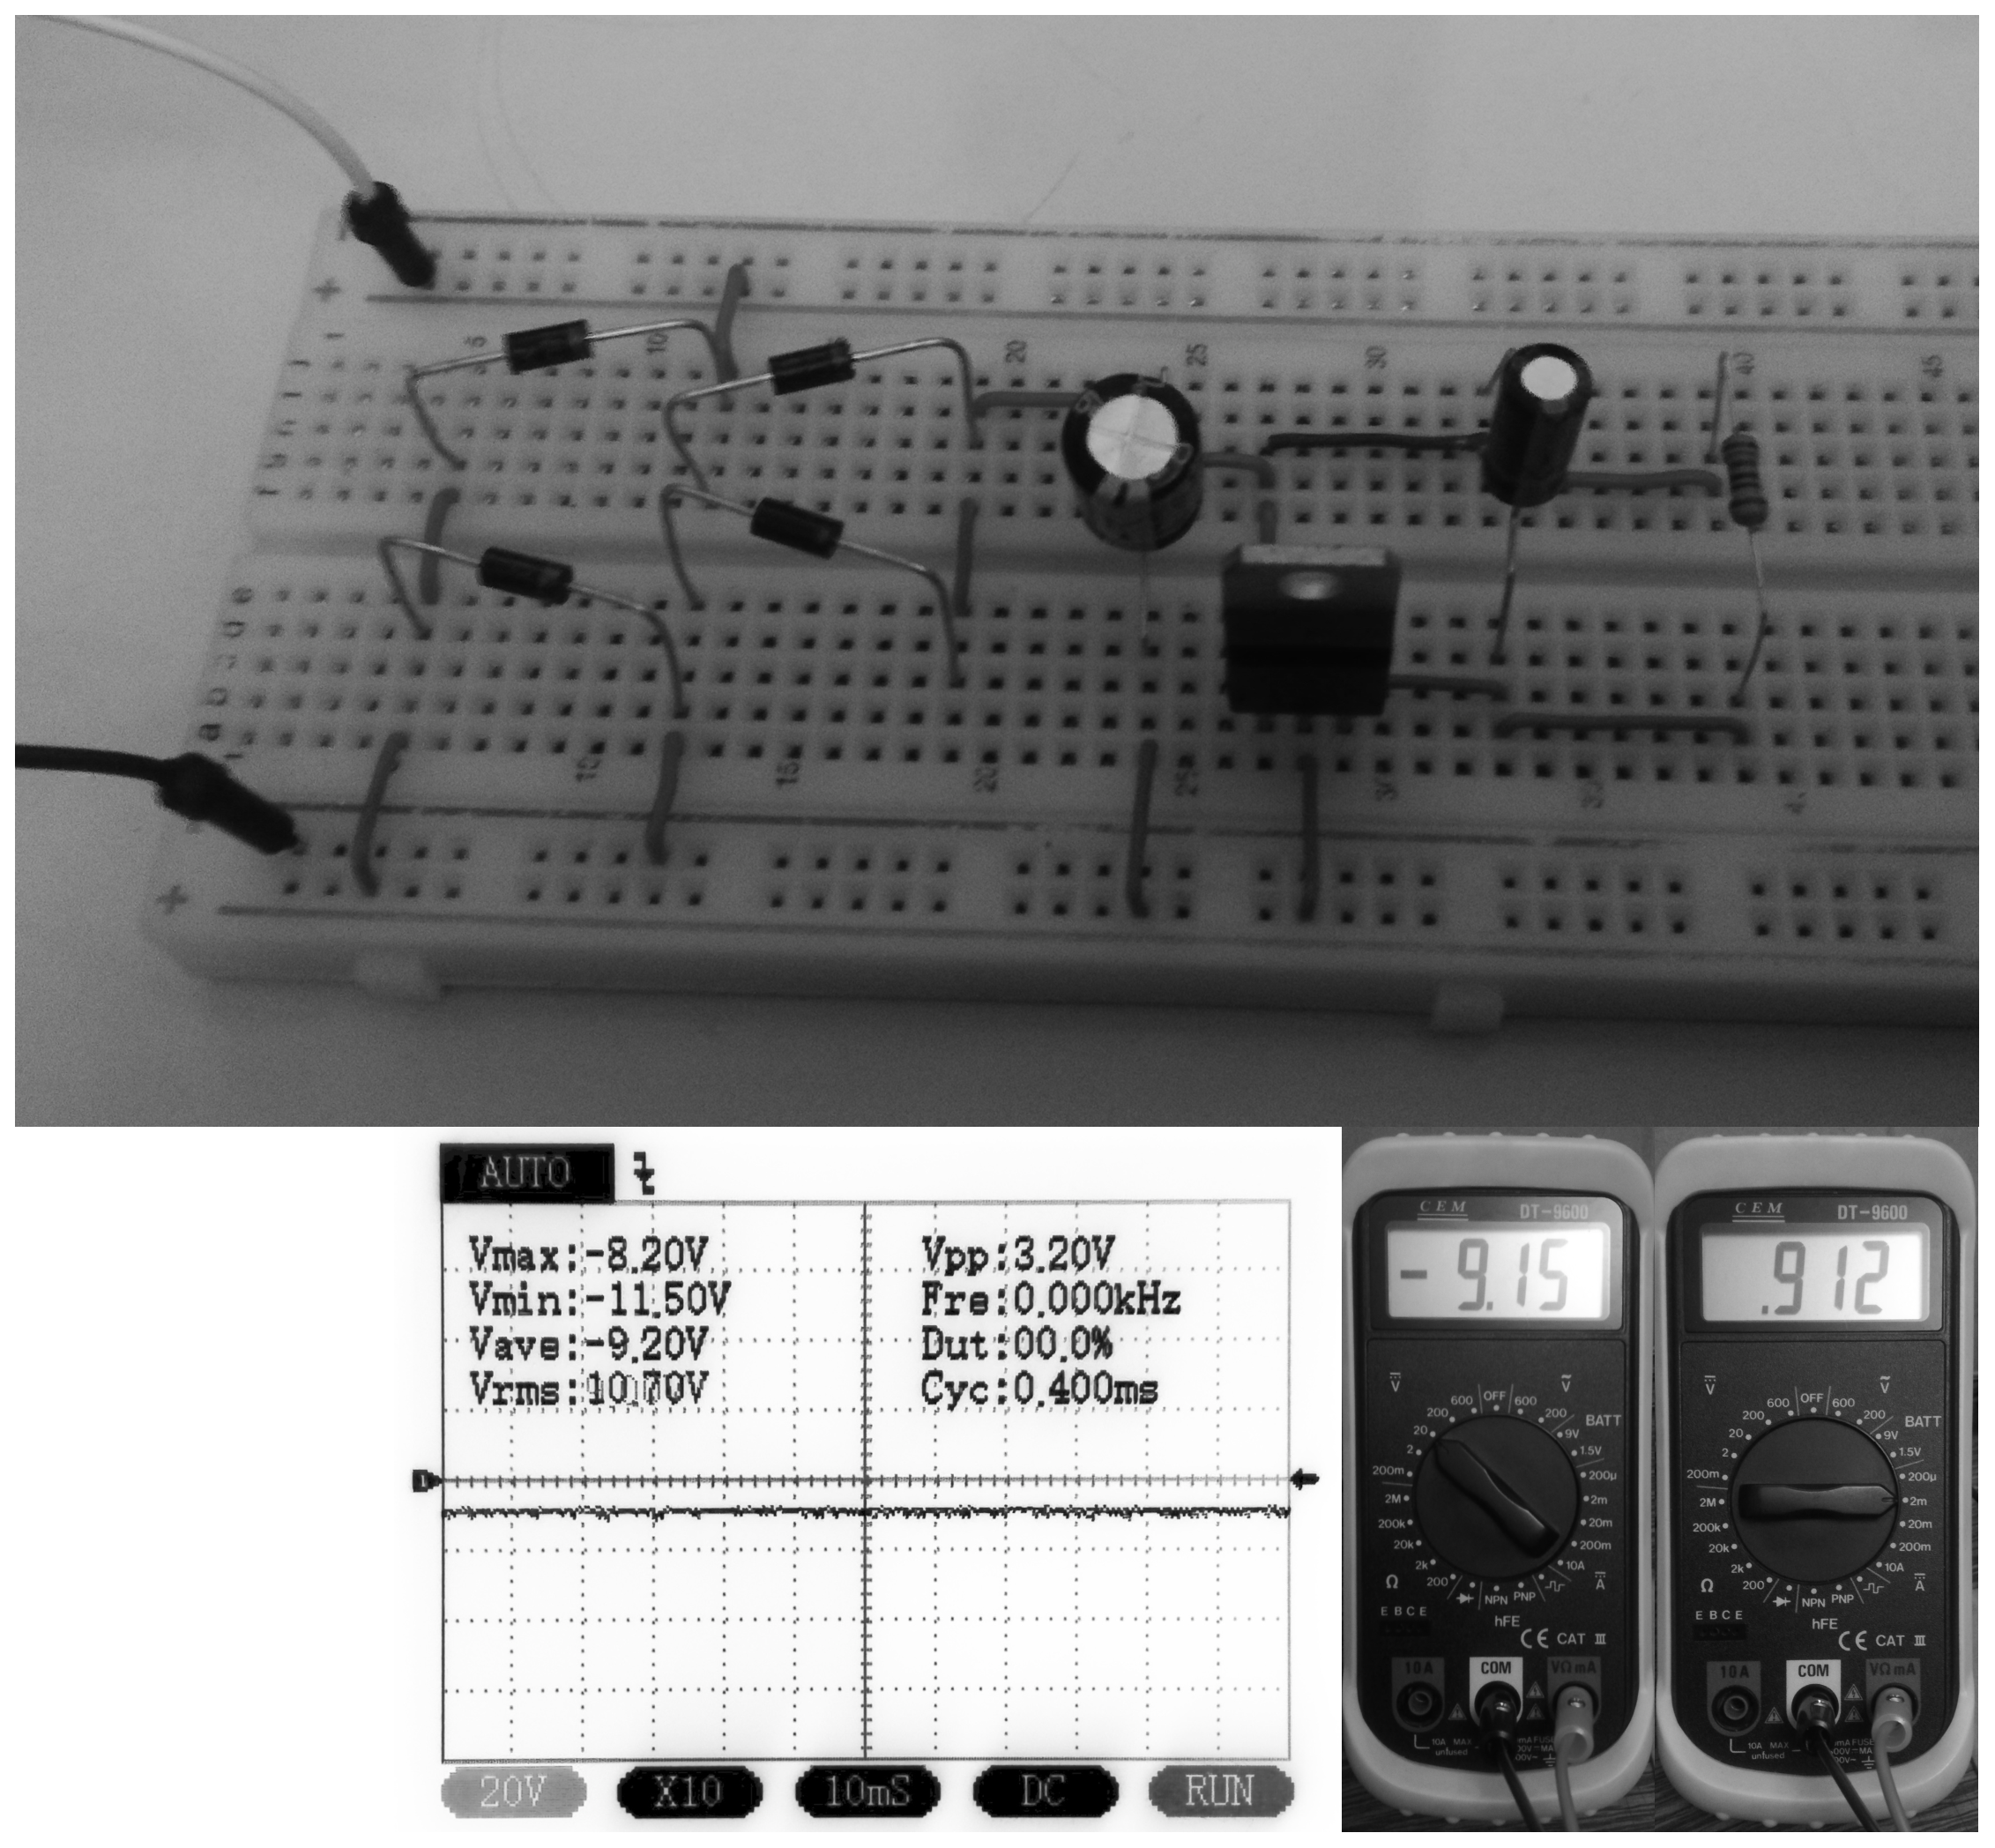
\includegraphics[scale=0.28]{fotos/10.regulador2.eps}
\caption{Regulador \textbf{L7909CV}, salida del osciloscopio\\
y medicion de voltaje y corriente.}
\label{laboratorio12}
\end{figure}

\subsection{Combinación de reguladores L7809CV y L7909CV}
Es posible combinar ambos reguladores positivo y negativo para incrementar la
salida de voltaje, como se muestra en la \textbf{figura~\ref{circuito11}}.

\begin{figure}[!h]
\centering
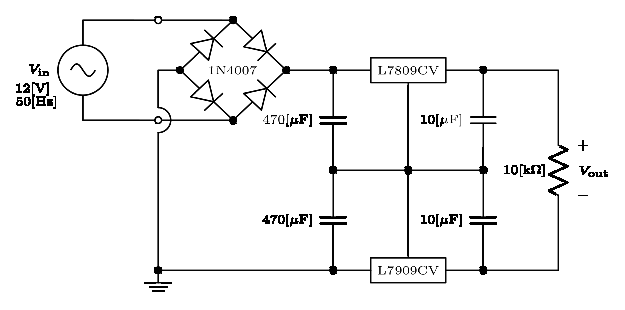
\includegraphics[scale=1.20]{diagramas/11.regulador3.eps}
\caption{Regulación de voltaje con dos circuitos integrados.}
\label{circuito11}
\end{figure}

\subsubsection{Simulación}
Se utilizó el software \emph{Quite Universal Circuit Simulator.} versión 23.3.1
para la simulación de la regulación de voltaje por medio de dos rectificadores,
este puede verse en la \textbf{figura~\ref{simulacion11}}.

\begin{figure}[!h]
\centering
\includegraphics[scale=0.75]{simulacion/11.regulador3.eps}
\caption{Simulación del regulador combinado.}
\label{simulacion11}
\end{figure}

\subsubsection{Laboratorio}
Se presenta el regulador con dos circuitos integrados armado en laboratorio, su
señal de voltaje de salida en osciloscopio, asi como su voltaje y corriente en
un multimetro para una resistencia de carga de $10[\text{k}\Omega]$ en la
\textbf{figura~\ref{laboratorio13}}.

\begin{figure}[!h]
\centering
\includegraphics[scale=0.28]{fotos/11.regulador3.eps}
\caption{Regulador combinado, salida del osciloscopio\\
y medicion de voltaje y corriente.}
\label{laboratorio13}
\end{figure}

%\subsection{Regulación variable con L7890CV}

%\begin{figure}[!h]
%\centering
%\includegraphics[scale=1.20]{diagramas/12.regulador4.eps}
%\caption{Regulación de voltaje con resistencia variable.}
%\label{circuito11}
%\end{figure}

